\documentclass[border=15pt, multi, tikz]{standalone}
\usepackage{rotating}
\usepackage{import}
\subimport{./utils/}{init}
\usetikzlibrary{positioning}
\usetikzlibrary{3d} %for including external image 

\def\fConvColor{rgb:magenta,1;black,0.5}
\def\dConvColor{rgb:blue,1}
\def\pConvColor{rgb:blue,1;white,0.5;cyan,0.5}
\def\PoolColor{rgb:orange,1}

\def\Opacity{0.75}

\begin{document}
\begin{tikzpicture}
\tikzstyle{connection}=[ultra thick,every node/.style={sloped,allow upside down},draw=\edgecolor,opacity=\Opacity,]
%%%%%%%%%%%%%%%%%%%%%%%%%%%%%%%%%%%%%%%%%%%%%%%%%%%%%%%%%%%%%%%%%%%%%%%%%%%%%%%%%%%%%%%%
%% Draw Layer Blocks
%%%%%%%%%%%%%%%%%%%%%%%%%%%%%%%%%%%%%%%%%%%%%%%%%%%%%%%%%%%%%%%%%%%%%%%%%%%%%%%%%%%%%%%%
\node[canvas is zy plane at x=0] (temp) at (-4.75,0,0) {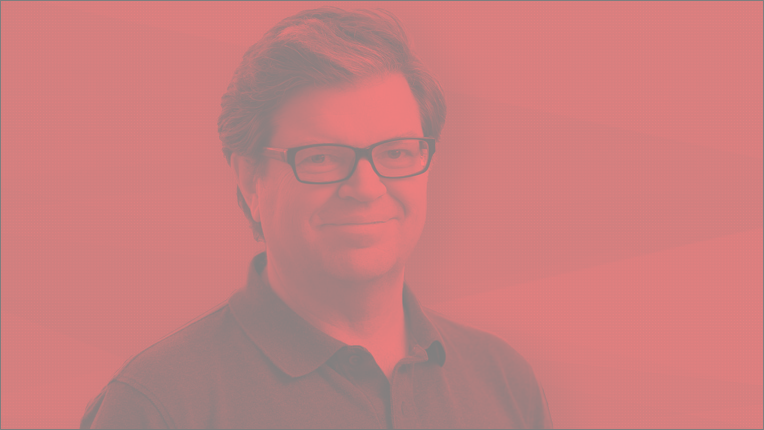
\includegraphics[width=8cm,height=8cm]{yann_red.png}};
\node[canvas is zy plane at x=0] (temp) at (-5,0,0) {
\includegraphics[width=8cm,height=8cm]{yann_green.png}};
\node[canvas is zy plane at x=0] (temp) at (-5.25,0,0) {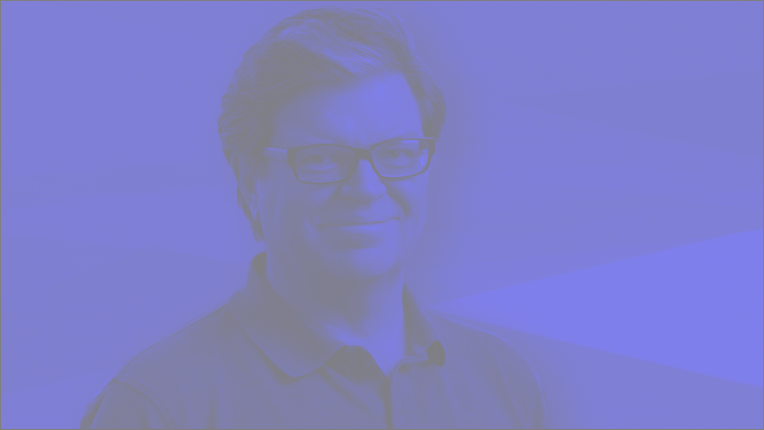
\includegraphics[width=8cm,height=8cm]{yann_blue.png}};

% conv1
\pic[shift={(0,0,0)}] at (0,0,0) {RightBandedBox={name=cr1,zlabel=224,position=-0.25,%
        xlabel={{"16",}},fill=\fConvColor,opacity=\Opacity,bandfill=\fConvColor,%
        height=40,width={2.773},depth=40}};
%pool1
\pic[shift={(0,0,0)}] at (cr1-east) {Box={name=p1,zlabel=112,position=0.4,%
        xlabel={"16",},fill=\PoolColor,opacity=\Opacity,height=30,width=2.773,depth=30}};


% conv2 and conv3
\pic[shift={(4,0,0)}] at (p1-east) {RightBandedBox={name=scr2,%
        xlabel={{"16",}},fill=\dConvColor,opacity=\Opacity,bandfill=\dConvColor,%
        height=30,width={2.773},depth=30}};
\pic[shift={(0,0,0)}] at (scr2-east) {RightBandedBox={name=cr2,zlabel=112,position=-0.25,%
        xlabel={{"32",}},fill=\pConvColor,opacity=\Opacity,bandfill=\pConvColor,%
        height=30,width={3.466},depth=30}};
%pool2
\pic[shift={(0,0,0)}] at (cr2-east) {Box={name=p2,zlabel=56,position=0.5,%
        xlabel={"32",},fill=\PoolColor,opacity=\Opacity,height=23.5,width=3.466,depth=23.5}};


% conv4 and conv5
\pic[shift={(3.5,0,0)}] at (p2-east) {RightBandedBox={name=scr3,%
        xlabel={{"32",}},fill=\dConvColor,opacity=\Opacity,bandfill=\dConvColor,%
        height=23.5,width={3.466},depth=23.5}};
\pic[shift={(0,0,0)}] at (scr3-east) {RightBandedBox={name=cr3,zlabel=56,position=-0.25,%
        xlabel={{"64",}},fill=\pConvColor,opacity=\Opacity,bandfill=\pConvColor,%
        height=23.5,width={4.159},depth=23.5}};
%pool3
\pic[shift={(0,0,0)}] at (cr3-east) {Box={name=p3,zlabel=28,position=0.56,%
        xlabel={"64",},fill=\PoolColor,opacity=\Opacity,height=16.875,width=4.159,depth=16.875}};


% conv6 and conv7
\pic[shift={(3,0,0)}] at (p3-east) {RightBandedBox={name=scr4,%
        xlabel={{"64",}},fill=\dConvColor,opacity=\Opacity,bandfill=\dConvColor,%
        height=16.875,width={4.159},depth=16.875}};
\pic[shift={(0,0,0)}] at (scr4-east) {RightBandedBox={name=cr4,zlabel=28,position=-0.25,%
        xlabel={{"128",}},fill=\pConvColor,opacity=\Opacity,bandfill=\pConvColor,%
        height=16.875,width={4.852},depth=16.875}};
%pool4
\pic[shift={(0,0,0)}] at (cr4-east) {Box={name=p4,zlabel=14,position=0.7,%
        xlabel={"128",},fill=\PoolColor,opacity=\Opacity,height=12.65625,width=4.852,depth=12.65625}};


% conv8 and conv9
\pic[shift={(2.5,0,0)}] at (p4-east) {RightBandedBox={name=scr5,%
        xlabel={{"128",}},fill=\dConvColor,opacity=\Opacity,bandfill=\dConvColor,%
        height=12.65625,width={4.852},depth=12.65625}};
\pic[shift={(0,0,0)}] at (scr5-east) {RightBandedBox={name=cr5,zlabel=14,position=-0.25,%
        xlabel={{"256",}},fill=\pConvColor,opacity=\Opacity,bandfill=\pConvColor,%
        height=12.65625,width={5.545},depth=12.65625}};
%pool5
\pic[shift={(0,0,0)}] at (cr5-east) {Box={name=p5,zlabel=\begin{turn}{5}7\end{turn},position=1,%
        xlabel={"256",},fill=\PoolColor,opacity=\Opacity,height=9.492,width=5.545,depth=9.492}};


% conv10 and conv11
\pic[shift={(2,0,0)}] at (p5-east) {RightBandedBox={name=scr6,%
        xlabel={{"256",}},fill=\dConvColor,opacity=\Opacity,bandfill=\dConvColor,%
        height=9.492,width={5.545},depth=9.492}};
\pic[shift={(0,0,0)}] at (scr6-east) {NewBox={name=cr6,position=0,%
        xlabel={{"512",}},fill=\pConvColor,opacity=\Opacity,bandfill=\pConvColor,%
        height=9.492,width={6.238},depth=9.492}};
%pool6
\pic[shift={(0,0,0)}] at (cr6-east) {Box={name=p6,zlabel=\begin{turn}{5}7\end{turn},position=1,%
        xlabel={"512",},fill=\PoolColor,opacity=\Opacity,height=9.492,width=6.238,depth=9.492}};


% conv12
\pic[shift={(3,0,0)}] at (p6-east) {NewBox={name=cr7,zlabel=\begin{turn}{5}7\end{turn},position=-0.25,%
        xlabel={{"25",}},fill=\pConvColor,opacity=\Opacity,bandfill=\pConvColor,%
        height=9.492,width={3.219},depth=9.492}};

\node[] at (32,5.5,0) {\Large\textcolor{\fConvColor}{Purple: Full Convolution}};
\node[] at (32,5,0) {\Large\textcolor{\dConvColor}{Dark Blue: Depthwise Convolution}};
\node[] at (32,4.5,0) {\Large\textcolor{\pConvColor}{Light Blue: Pointwise Convolution}};
\node[] at (32,4,0) {\Large\textcolor{\PoolColor}{Orange: Max Pooling}};
\node[] at (16.5,5.5,0) {\Large{Conv \& Pool Key: kernelType [kw,hw,inchan]/stride $\times$ outchan}};
\node[] at (16.5,5,0) {\Large{Layer Dimension Key: width $\times$ height $\times$ channels}};

\node[] at (-5,-7,0) {\large{Input Image}};
\node[] at (-5,-7.5,0) {\large{R, G, B Channels}};
\node[] at (-5,-8,0) {\large{224$\times$224$\times$3}};

\node[] at (0,-7,0) {\large\textcolor{\fConvColor}{conv1: [3,3,3]/1 $\times$ 16}};
\node[] at (0,-7.5,0) {\large\textcolor{\fConvColor}{224$\times$224$\times$16}};
\node[] at (0,-8.25) {\large\textcolor{\PoolColor}{max1: [2,2,1]/2 $\times$ 16}};
\node[] at (0,-8.75,0) {\large\textcolor{\PoolColor}{112$\times$112$\times$16}};

\node[] at (5.75,-5.5,0) {\large\textcolor{\dConvColor}{conv2: [3,3,1]/1 $\times$ 16}};
\node[] at (5.75,-6,0) {\large\textcolor{\dConvColor}{112$\times$112$\times$16}};
\node[] at (5.75,-6.75,0) {\large\textcolor{\pConvColor}{conv3: [1,1,16]/1 $\times$ 32}};
\node[] at (5.75,-7.25,0) {\large\textcolor{\pConvColor}{112$\times$112$\times$32}};
\node[] at (5.75,-8,0) {\large\textcolor{\PoolColor}{max2: [2,2,1]/2 $\times$ 32}};
\node[] at (5.75,-8.5,0) {\large\textcolor{\PoolColor}{56$\times$56$\times$32}};

\node[] at (11.5,-4.5,0) {\large\textcolor{\dConvColor}{conv4: [3,3,1]/1 $\times$ 32}};
\node[] at (11.5,-5,0) {\large\textcolor{\dConvColor}{56$\times$56$\times$32}};
\node[] at (11.5,-5.75,0) {\large\textcolor{\pConvColor}{conv5: [1,1,32]/1 $\times$ 64}};
\node[] at (11.5,-6.25,0) {\large\textcolor{\pConvColor}{56$\times$56$\times$64}};
\node[] at (11.5,-7,0) {\large\textcolor{\PoolColor}{max3: [2,2,1]/2 $\times$ 64}};
\node[] at (11.5,-7.5,0) {\large\textcolor{\PoolColor}{28$\times$28$\times$64}};

\node[] at (17,-4,0) {\large\textcolor{\dConvColor}{conv6: [3,3,1]/1 $\times$ 64}};
\node[] at (17,-4.5,0) {\large\textcolor{\dConvColor}{28$\times$28$\times$64}};
\node[] at (17,-5.25,0) {\large\textcolor{\pConvColor}{conv7: [1,1,64]/1 $\times$ 128}};
\node[] at (17,-5.75,0) {\large\textcolor{\pConvColor}{28$\times$28$\times$128}};
\node[] at (17,-6.5,0) {\large\textcolor{\PoolColor}{max4: [2,2,1]/2 $\times$ 128}};
\node[] at (17,-7,0) {\large\textcolor{\PoolColor}{14$\times$14$\times$128}};

\node[] at (22.5,-3.5,0) {\large\textcolor{\dConvColor}{conv8: [3,3,1]/1 $\times$ 128}};
\node[] at (22.5,-4,0) {\large\textcolor{\dConvColor}{14$\times$14$\times$128}};
\node[] at (22.5,-4.75,0) {\large\textcolor{\pConvColor}{conv9: [1,1,128]/1 $\times$ 256}};
\node[] at (22.5,-5.25,0) {\large\textcolor{\pConvColor}{14$\times$14$\times$256}};
\node[] at (22.5,-6,0) {\large\textcolor{\PoolColor}{max5: [2,2,1]/2 $\times$ 256}};
\node[] at (22.5,-6.5,0) {\large\textcolor{\PoolColor}{7$\times$7$\times$256}};

\node[] at (28,-3.5,0) {\large\textcolor{\dConvColor}{conv10: [3,3,1]/1 $\times$ 256}};
\node[] at (28,-4,0) {\large\textcolor{\dConvColor}{7$\times$7$\times$256}};
\node[] at (28,-4.75,0) {\large\textcolor{\pConvColor}{conv11: [1,1,256]/1 $\times$ 512}};
\node[] at (28,-5.25,0) {\large\textcolor{\pConvColor}{7$\times$7$\times$512}};
\node[] at (28,-6,0) {\large\textcolor{\PoolColor}{max6: [2,2,1]/1 $\times$ 512}};
\node[] at (28,-6.5,0) {\large\textcolor{\PoolColor}{7$\times$7$\times$512}};

\node[] at (33,-3.5,0) {\large\textcolor{\pConvColor}{conv12: [1,1,512]/1 $\times$ 25}};
\node[] at (33,-4,0) {\large\textcolor{\pConvColor}{7$\times$7$\times$25}};

\node[] at (26.5, -9 ,0) {{Layer depths are drawn with logarithmic scaling. Max pooling layer widths and heights are shrunk by $\frac{1}{4}$ instead of $\frac{1}{2}$.}};

%%%%%%%%%%%%%%%%%%%%%%%%%%%%%%%%%%%%%%%%%%%%%%%%%%%%%%%%%%%%%%%%%%%%%%%%%%%%%%%%%%%%%%%%
%% Draw Arrow Connections
%%%%%%%%%%%%%%%%%%%%%%%%%%%%%%%%%%%%%%%%%%%%%%%%%%%%%%%%%%%%%%%%%%%%%%%%%%%%%%%%%%%%%%%%
% \draw [connection]  (p1-east)        -- node {\midarrow} (cr2-west);
% \draw [connection]  (p2-east)        -- node {\midarrow} (cr3-west);
% \draw [connection]  (p3-east)        -- node {\midarrow} (cr4-west);
% \draw [connection]  (p4-east)        -- node {\midarrow} (cr5-west);
% \draw [connection]  (p5-east)        -- node {\midarrow} (fc6-west);
% \draw [connection]  (fc6-east)       -- node {\midarrow} (fc7-west);
% \draw [connection]  (fc7-east)       -- node {\midarrow} (fc8-west);
% \draw [connection]  (softmax-east)   -- node {\midarrow} ++(1.5,0,0);
%%%%%%%%%%%%%%%%%%%%%%%%%%%%%%%%%%%%%%%%%%%%%%%%%%%%%%%%%%%%%%%%%%%%%%%%%%%%%%%%%%%%%%%%
%% Draw Dotted Edges 
%%%%%%%%%%%%%%%%%%%%%%%%%%%%%%%%%%%%%%%%%%%%%%%%%%%%%%%%%%%%%%%%%%%%%%%%%%%%%%%%%%%%%%%%

%%%%%%%%%%%%%%%%%%%%%%%%%%%%%%%%%%%%%%%%%%%%%%%%%%%%%%%%%%%%%%%%%%%%%%%%%%%%%%%%%%%%%%%%
\end{tikzpicture}
\end{document}